\documentclass[11pt]{article} \usepackage[top=1in, bottom=1in, left=1in, right=1in]{geometry}
\usepackage{amsfonts, amsmath, amssymb, amsthm}
\usepackage{xcolor}
\usepackage{hyperref}
\usepackage[british,calc]{datetime2}
\usepackage{advdate}
\usepackage{tikz}
\usepackage{booktabs}

\usetikzlibrary{calc,arrows}

% Timeline https://tex.stackexchange.com/questions/61237/timeline-and-tikz
\newdimen\XCoord
\newdimen\YCoord
\newcommand*{\ExtractCoordinate}[1]{\path (#1); \pgfgetlastxy{\XCoord}{\YCoord};}
% modify these for altered timeline appearance
% ============================= 
\pgfmathsetmacro{\mintime}{0}
\pgfmathsetmacro{\maxtime}{14}
\newcommand{\timeunit}{Week}
\pgfmathtruncatemacro{\timeintervals}{14}
\pgfmathsetmacro{\scaleitemseparation}{3}
\pgfmathsetmacro{\timenodewidth}{8cm}
\newcounter{itemnumber}
\setcounter{itemnumber}{0}
\newcommand{\lastnode}{n-0}
% ============================= 
% entry in timeline
\newcommand{\timeentry}[2]{% time, description
\stepcounter{itemnumber}
\node[below right,text width=\timenodewidth] (n-\theitemnumber) at (\lastnode.south west) {#2};
\edef\lastnode{n-\theitemnumber}
\expandafter\edef\csname nodetime\theitemnumber \endcsname{#1}
}
% timeline scale and labels
\newcommand{\drawtimeline}[1]{% start date
    \draw[very thick,-latex] (0,0) -- ($(\lastnode.south west)-(\scaleitemseparation,0)+(0,-1)$);
    \ExtractCoordinate{n-\theitemnumber.south}
    \pgfmathsetmacro{\yposition}{\YCoord/28.452755}
    \foreach \x in {1,...,\theitemnumber}
    {   \pgfmathsetmacro{\timeposition}{\yposition/(\maxtime-\mintime)*\csname nodetime\x \endcsname}
        %\node[right] at (0,\timeposition) {\yposition};
        \draw (0,\timeposition) -- (0.5,\timeposition) -- ($(n-\x.west)-(0.5,0)$) -- (n-\x.west);
    }
    \foreach \x in {0,...,\timeintervals}
    {   \pgfmathsetmacro{\labelposition}{\yposition/(\maxtime-\mintime)*\x}
        \node[left] (label-\x) at (-0.2,\labelposition) {\textcolor{gray}{\bf \timeunit\ \the\numexpr\x + 1\relax} \ \DTMdate{#1 + \the\numexpr\x * 7\relax}\ -\ \DTMdate{#1 + \the\numexpr\x * 7 +6\relax}};
        \draw (label-\x.east) -- ++ (0.2,0.0);
    }   
}

% set date format as mm//dd
\renewcommand{\DTMdisplaydate}[4]{#2/#3}

\renewcommand{\refname}{Reading List}

\title{Surgical Phase Detection Using Deep Learning\\ Proposal \& Plan}
\author{Xiaorui Zhang, Wenkai Luo, Xucheng Ma}
\date{February 2022}

\begin{document}

\maketitle

\section{Stated topic and goal}
Surgical phase recognition plays a crucial role in the era of digitized surgery. Deep learning solutions have seen great success in endoscopic surgeries. Currently, no prior work has investigated its application in skull-base surgery (Cortical Mastoidectomy). This project will benchmark existing DL solutions and create an innovative DL segmentation algorithm in skull-based surgery.

\section{Team members, mentor}
\begin{itemize}
    \item \textbf{Students}:\\Xucheng Ma, Xiaorui Zhang, Wenkai Luo
    \item \textbf{Mentors}:\\Max Li, Danielle Trakimas, Dr.Francis Creighton, Prof. Mathias Unberath, Prof. Russ Taylor
\end{itemize}

\section{Relevance/importance}
Surgical phase recognition has numerous potential medical applications. Such as automatic indexing of surgical video databases and real-time operating room scheduling optimization. It’s also a foundation of an intelligent context-aware system, which facilitates surgery monitoring, surgical protocol extraction, and decision support. To be more specific on our project, Mastoidectomy is a highly delicate and complex surgery. There are many facial nerves and blood vessels around the region of operation. It would be ideal for the surgeon to have an intelligent context-awareness system to facilitate decision-making. Our online video segmentation model would be necessary for this system to be aware of the current surgical phase. 
\section{Short technical summary of approach}
Instead of considering surgical phase segmentation as a per-frame classification, we take the entire surgical video as input, utilize both spatial and temporal features, and solve as a sequence-to-sequence problem: sequence of image frame to sequence of surgical phase label. Spatial features describes underlying geometric characteristics of the anatomy and tool presence, and they serves as an embedding of the raw images. Sequence of spatial feature embeddings are then fed into temporal features extractor, where temporal features such as change in anatomy and tool movement are extracted. Finally, a high-level classifier takes the spatial-temporal features as input and output surgical phase labels.
\begin{itemize}
    \item \textit{Spatial feature extraction:}\\
    One of the essential parts of the architecture is the spatial feature extractor, which extracts the feature from the frames and converts them into an abstract representation format. Based on the idea of transfer learning, the pre-trained convolutional neural network(CNN) models have been proved to be stat-of-the-art on many computer vision tasks. Furthermore, the pre-trained model can extract more specific features with the fine-tuning process using the mastoidectomy dataset. 
    \item \textit{Temporal feature extraction:}\\
   The most crucial part of the architecture is the temporal feature extraction, which captures the temporal patterns from the extracted per-frame spatial features from video. The temporal patterns are essential to correct surgical phase prediction since the patterns often provide clues of surgery environment change and the instrument motion. Recurrent neural networks such as LSTM, temporal convolution neural network (TCN), and transformer are promising architectures for capturing the temporal pattern. However, some research argues that LSTM can only capture short-term information while long-term context might be beneficial for accurate segmentation. All of them will be implemented on the mastoidectomy dataset in our project.
   \item \textit{High-level Classifier:}\\
   The fully connected neural network(FCNN) will then be trained with the ground truths to make the phase decision based on the extracted spatiotemporal feature since it can approximate any arbitrary function. One crucial concern is the over-fitting issue, which can be compensated by different training skills such as drop-out and batch-normalization. 
\end{itemize}

\section{Deliverables}
Project deliverables are listed as follows:
\begin{itemize}
    \item \textbf{Minimum Deliverables}
    \begin{itemize}
        \item New dataset from cortical mastoidectomy videos (with Danielle's help)
        \item At least three methods
        \item All methods trained and evaluated on the new dataset
    \end{itemize}
    \item \textbf{Expected Deliverables}
    \begin{itemize}
        \item Experiments and comparison with existing methods
        \item Ablation study
    \end{itemize}
    \item \textbf{Maximum Deliverables}
    \begin{itemize}
        \item Conference paper
    \end{itemize}
\end{itemize}

\section{Timeline \& Milestones}
Figure \ref{fig:timeline} shows the project timeline. \textcolor{blue}{Milestones} are labeled in blue, and deadlines for resolving \textcolor{red}{dependencies} are labeled in red. Other entries in the timeline indicate either start point or end point of tasks.
\begin{figure}[!ht]
    \centering
    \begin{tikzpicture}
        \node[inner sep=0] (n-0) at (\scaleitemseparation,0) {};
        \timeentry{0.5}{Literature review}
        \timeentry{1.5}{Proposal and plan}
        \timeentry{2}{Start data annotations, environment setup}
        \timeentry{2.6}{\textcolor{blue}{\bf Proposal and Plan Presentation}}
        \timeentry{3.4}{\textcolor{red}{\bf Sample Dataset} }
        \timeentry{3.6}{Finish environment setup}
        \timeentry{4.5}{Start data-prepocession for \\ benchmark methods}
        \timeentry{5.5}{Start implementing model evaluation}
        \timeentry{6.5}{Ready to training benchmart methods}
        \timeentry{7.2}{\textcolor{red}{\bf Computational resources}}
        \timeentry{7.3}{\textcolor{red}{\bf Fullly annotated dataset}}
        \timeentry{7.4}{\textcolor{blue}{\bf Seminar Presentation}}
        \timeentry{7.6}{Benchmark methods training}
        \timeentry{8.5}{\textcolor{blue}{\bf Minimum Deliverables}}
        \timeentry{9.3}{\textcolor{blue}{\bf Checkpoint Presentation}}
        \timeentry{9.7}{\textcolor{blue}{\bf Initial design of improved method}}
        \timeentry{10.5}{Train and evaluate improved method}
        \timeentry{11.5}{\textcolor{blue}{\bf Expected Deliverables}}
        \timeentry{12.5}{Poster and final report}
        \timeentry{13.5}{Additional experiments}
        \timeentry{14}{\textcolor{blue}{\bf Final presentation}}
        \drawtimeline{2022-1-24}
    \end{tikzpicture}
    \caption{Project timeline, \textcolor{blue}{Milestones} labeled in \textcolor{blue}{blue}, \textcolor{red}{Deliverables deadline} labeled in \textcolor{red}{red}}
    \label{fig:timeline}
\end{figure}

\section{List of dependencies \& plan for resolving}

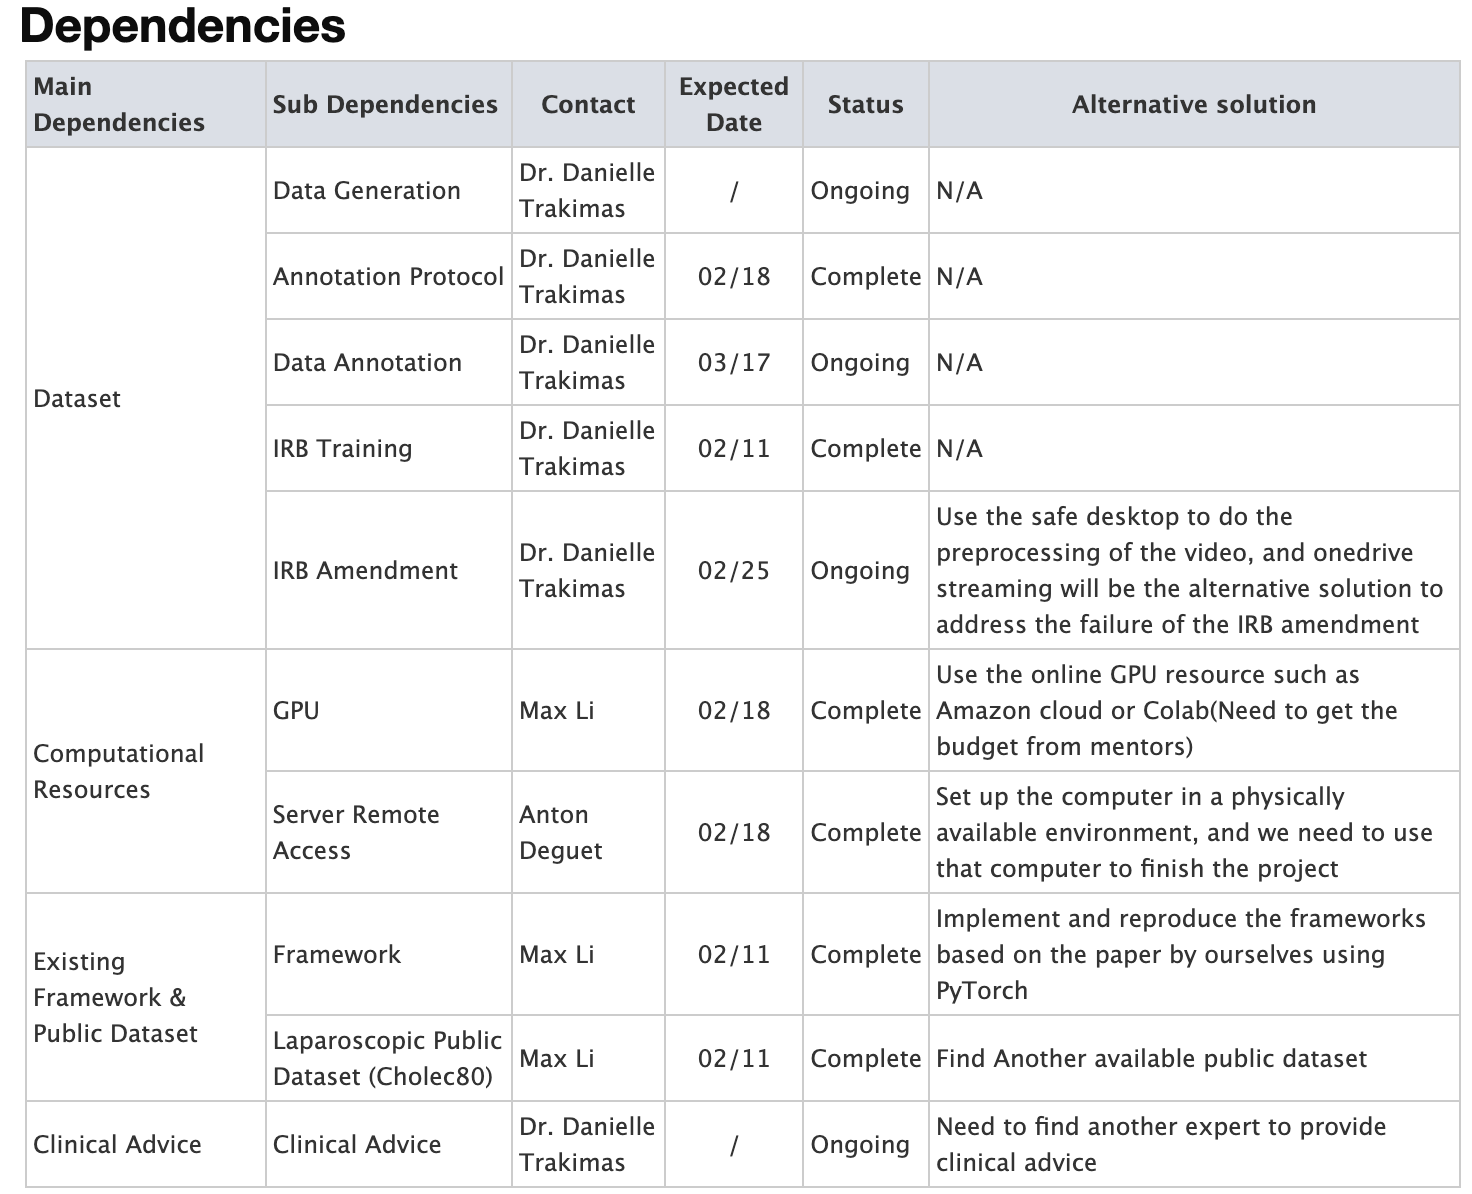
\includegraphics[width=\textwidth]{dependency.png}

\section{Management Plan}
\begin{itemize}
    \item We meet with our mentors and report weekly progress every Friday.
    \item Slack are used for daily communication.
    \item All project relevent codes and documentation are managed with git.
    \item Project progress is monitored with Gantt Chart. 
\end{itemize}
\nocite{*}
\bibliographystyle{unsrt}
\bibliography{bibfile}

\end{document}
